% Fonte tamanho 11, duas colunas, tipo artigo.
\documentclass[11pt]{article}

% Escrita em português
\usepackage[utf8]{inputenc}
\usepackage[T1]{fontenc}
\usepackage[portuges, english]{babel}

% Inclusão de Imagens
\usepackage{graphicx}

% Correção de Margens
\usepackage
[
        top = 2.5cm,
        left = 2.5cm,
        right = 2.5cm,
        bottom = 2.5cm
]{geometry}

% Símbolos Matemáticos
\usepackage{amsmath}
\usepackage{mathrsfs}
% Altera sin(x) para sen(x)
\def\sen{\mathop{\mbox{\normalfont sen}}\nolimits}

% Unidades do SI
\usepackage{siunitx}

% Tabelas
\usepackage{booktabs}
\usepackage{array}
\usepackage{multirow}
\usepackage[table, dvipsnames]{xcolor}

% Figuras lado-a-lado
\usepackage{caption}
\usepackage{subcaption}

% Bibliografia
\usepackage
[
        style     = ieee,
        citestyle = numeric
]{biblatex}
\bibliography{bibliography.bib}


% Pacotes de rascunho
\usepackage{lipsum}

% Variáveis de informação
% Título
\newcommand{\vartitulo}{Método dos Mínimos Quadrados aplicado
                        no ajuste dos pesos de notas para
                        disciplinas acadêmicas}
% Nome (Formato A. B. C. Sobrenome)
\newcommand{\varautor}{A. B. C. Sobrenome}
% Instituição de Ensino
\newcommand{\varinstituicao}{Universidade Universidade}
% Departamento
\newcommand{\vardepartamento}{Departamento de Departamento}
% Informações de contato
\newcommand{\varcontato}{Caixa Postal: XXXXX -
                         CEP: XXXXX-XXX -
                         Cidade -
                         Estado \\
                         Fone: +XX-XX-XXXX-XXXX -
                         Fax: +XX-XX-XXXX-XXXX \\
                         email@de.contato}

% Informações para o título
\title{\vartitulo}
\author
{
        \varautor \\
        \varinstituicao \\
        \vardepartamento \\
        \varcontato
}
\date{}

\begin{document}
        \selectlanguage{portuges}
        \sisetup{output-decimal-marker = {,}}
% Informações autorais e de contato
        \maketitle

% Resumo do trabalho
        \abstract
        {
                % Coloque aqui o resumo do trabalho
                Estuda-se a viabilidade do uso do Método de
                Mínimos Quadrados para o ajuste dos pesos
                referentes ao cálculo de notas de uma
                disciplina acadêmica, de modo a maximizar
                o desempenho dos estudantes. São analisadas duas
                configurações principais relativas ao número de
                variáveis livres (pesos) na composição da nota,
                mostrando a aplicabilidade do método, em
                especial nos casos em que há poucas
                variáveis, além de como
                \begin{otherlanguage}{english}
                        \textit{outliers}
                \end{otherlanguage}
                afetam as grandezas de análise de desempenho
                geral (média da turma e distribuição de
                alunos aprovados/em exame final/reprovados)
                para cada uma das configurações.
                \newline

                % Palavras Chave
                Palavras-chave:
                Ajuste de pesos,
                Barreira de domínio,
                Cálculo de notas,
                Maximização de desempenho estudantil,
                Método dos Mínimos Quadrados.

                % Espaço livre
                \vspace{2\baselineskip}
        }



% Objetivo
        \section{Objetivo}
		Nesse trabalho, por meio do Método de Mínimos
		Quadrados, determinaram-se os pesos para o
		ajuste das notas de Física Básica Experimental
		2, de modo a maximizar, na média, o
                desempenho dos estudantes.

% Fundamentação Teórica
        \section{Fundamentação Teórica}
		As notas da matéria se dividem em relatórios e
		provas. Até o momento de escrita desse trabalho,
		dispunhamos apenas das notas de dois dos três
		relatórios e provas realizados para o semestre,
		contudo, estabelecida a validade e a praticidade
		do seguinte método para tal aplicação como
		forma de
		\begin{otherlanguage}{english}
			\textit{proof of concept}
		\end{otherlanguage}
		pode-se então aplicá-lo, mantida a
		infraestrutura computacional, de maneira ágil
		para a coleção completa das notas do semestre.

		Foram estudados duas configurações de pesos, em
		uma delas, tomamos todos os pesos de cada uma
		das avaliações como independentes, em outra,
		consideramos apenas o peso da média
		aritméticas dos relatórios e da
                média aritmética das provas. A análise
                da fundamentação matemática se dará para esse
                caso, em virtude de sua simplificada
                descrição, em termos do número de
                símbolos empregados. A análise para os pesos
                independentes, pode ser feita de forma
                completamente análoga, e sua formulação final
                pode ser vista na
                Equação~\ref{SISTEMA_PESOS_INDEPENDENTES}.

		Considerando as notas $P$ e $R$, relativas
                à média artimética das provas e dos relatórios,
                respectivamente, e seus pesos correspondentes
                $P_P$ e $P_R$, a média final pode ser calculada
                por uma média ponderada, da forma
                \begin{equation}
                        N_F =
			\frac{P_{P}P + P_{R}R}
			     {P_{P} + P_{R}}
                        \label{MEDIA_PONDERADA}
                \end{equation}
		e, deseja-se tentar aproximar, para todos os
		alunos, a nota $N_F$ de $10$. Isto é, haverá
		um sistema com linhas do tipo
                \begin{equation*}
			P_{P}P + P_{R}R =
			10\cdot
			  \left(
			  P_{P} + P_{R}
			  \right)
                \end{equation*}
		combinando fatores múltiplos do mesmo peso,
		é obtido
                \begin{equation*}
                        P_{P}(P - 10) + P_{R}(R - 10) = 0
                \end{equation*}
                onde desejam-se ajustar os pesos $P_{P}$ e
                $P_{R}$ de forma a aproximar, para todos os
                alunos, essa igualdade ao máximo.
		Entretanto, esse formato tem um problema: A
		solução trivial é sempre solução, portanto o
		método de mínimos quadrados sempre produziria,
		para o vetor de resultados, o vetor nulo.

		Identificou-se como a origem do problema a
		inserção de um grau de liberdade que não está
		realmente presente, isto é, pode-se reduzir o
		problema estabelecendo uma restrição em um dos
		pesos, como, por exemplo, o peso $P_{R2}$, de
		forma que a soma de todos os pesos seja sempre
		$1$. Isso permite reescrever a
                Equação~\ref{MEDIA_PONDERADA} como
                \begin{equation*}
                        N_F = P_{P}P + (1 - P_{P})R
                        \label{MEDIA_PONDERADA}
                \end{equation*}
                e, ao aproximar a nota final $N_F$ ao máximo
                para todos os indivíduos, resolve-se um
                sistema do tipo
		\begin{equation}
			P_{N}(P - R) =  10 - R.
			\label{SISTEMA_PESOS_SIMPLES}
		\end{equation}

		O caso com os $4$ pesos independentes também
                apresenta, ao tentar ajustar todos os pesos, a
                solução trivial. Novamente,
                se emprega uma solução análoga, fixando-se
                a soma dos pesos como unitária, permitindo
                reescrever o problema de mínimos quadrados como
                uma aproximação, para todos os alunos, de
                igualdades da forma
		\label{SISTEMA_PESOS_SIMPLES}
		se torna
		\begin{equation}
				P_{R1}(R_1 - P_2) +
				P_{R2}(R_2 - P_2) +
				P_{P1}(P_1 - P_2) = 10 - P_2
			\label{SISTEMA_PESOS_INDEPENDENTES}
		\end{equation}
		onde $R1$, $R2$, $P_{R1}$ $P_{R2}$ são as notas
		e os pesos dos relatórios $1$ e $2$,
		respectivamente, e $P_1$ e $P_{P1}$ são a nota
		e o peso da primeira prova. $P_2$ é a nota da
		segunda prova.

% Procedimento
        \section{Procedimento}
                Estabelecida a equação a ser aproximada de
                maneira geral para todos os alunos, exprimiu-a
                em termos de um sistema linear, da forma,
                para o caso da
                Equação~\ref{SISTEMA_PESOS_SIMPLES}
                \begin{equation}
                        \begin{bmatrix}
                                (P^1 - R^1) \\
                                \vdots      \\
                                (P^N - R^N) \\
                        \end{bmatrix}
                        \begin{bmatrix}
                                P_P
                        \end{bmatrix}
                        =
                        \begin{bmatrix}
                                (10 - R^1) \\
                                \vdots      \\
                                (10 - R^N) \\
                        \end{bmatrix}
                        \label{LINEAR_PESOS_SIMPLES}
                \end{equation}
                em que os sobrescritos são índices referindo
                aos alunos $1,2,\cdots,N$. No caso da
                Equação~\ref{SISTEMA_PESOS_INDEPENDENTES},
                o sistema linear toma uma forma mais
                complexa, porém similar
                \begin{equation}
                        \begin{bmatrix}
                                (P_{1}^1 - P_{2}^1) &
                                (R_{1}^1 - P_{2}^1) &
                                (R_{2}^1 - P_{2}^1)   \\
                                & \vdots &            \\
                                (P_{1}^N - P_{2}^N) &
                                (R_{1}^N - P_{2}^N) &
                                (R_{2}^N - P_{2}^N)   \\
                        \end{bmatrix}
                        \begin{bmatrix}
                                P_{P1} \\
                                P_{R1} \\
                                P_{R2} \\
                        \end{bmatrix}
                        =
                        \begin{bmatrix}
                                (10 - R^1) \\
                                \vdots      \\
                                (10 - R^N) \\
                        \end{bmatrix}.
                        \label{LINEAR_PESOS_INDEPENDENTES}
                \end{equation}

                Um fator que pode ser levado em conta nessas
                condições envolveu a exclusão de algumas
                entradas com base em algum fator discriminante,
                refazendo então o método de mínimos quadrados.
                Ilustrativamente, foram calculadas as
                configurações de peso, em ambos os modelos,
                levando em conta um limiar mínimo variável
                para a média aritmética das notas das provas.
                Isso foi feito pois possibilita um estudo da
                forma em que alunos com menor envolvimento na
                disciplina (o parâmetro para medir o
                envolvimento sendo, nesse caso, a média das
                provas) afetam os resultados do processo.

                De maneira direta, o procedimento pode ser
                subdividido em quatro etapas
                \begin{enumerate}
                        \item Calcular a configuração de
                              maximização dos pesos;
                        \item Incrementar um parâmetro limiar
                              para consideração das notas;
                        \item Excluir as notas referentes aos
                              alunos cuja média aritmética das
                              provas esteja abaixo desse limiar;
                        \item Se restaram alunos suficientes,
                              retornar ao item 1.
                \end{enumerate}
                Esse procedimento foi implementado
                computacionalmente utilizando decomposição
                QR por rotações em um código na
                linguagem C++.

                Assim, para cada um dos valores limiares,
                e para ambas as configurações, além dos próprios
                pesos foram também calculadas a média final
                da turma e a distribuição de alunos
                aprovados/em exame final/reprovados, de forma
                que os pesos fossem traduzidos para grandezas
                mais tangíveis.

                É evidente também que a resolução dos problemas
                de mínimos quadrados capturados nas
                Equações~\ref{SISTEMA_PESOS_SIMPLES} e
                \ref{SISTEMA_PESOS_INDEPENDENTES} não impõe
                qualquer limitação a respeito dos valores
                finais que os pesos podem assumir e,
                por isso,
                surgem pesos negativos e pesos
                maiores do que $1$, fazendo com que alunos
                possam ter médias finais maiores do que $10$
                ou ainda que um aluno com notas maiores
                tenha uma média final menor do que outro
                aluno que, contraditoriamente, teve, em
                todas as avaliações, notas menores.

                No caso da configuração em que existem apenas
                dois pesos, esse problema pode ser enfrentado
                por um passo extra no cálculo dos dados que
                foi denominado como
                \textbf{barreira de domínio},
                já que a Equação~\ref{MEDIA_PONDERADA} pode
                ser enxergada como uma função que, em
                condições ideais, recebe valores do intervalo
                fechado $[0,1]$, os pesos, e produz uma média
                final entre $0$ e $10$. Quando esses pesos,
                contudo, estavam fora desse domínio de
                validade, a barreira de domínio os levava
                para o valor válido mais próximos, isto é
                \begin{itemize}
                        \item Se o peso está acima de 1,
                              torne-o 1;
                        \item Se o peso está abaixo de 0,
                              torne-o 0;
                        \item Caso nenhum dos dois aconteça,
                              não modifique seu valor.
                \end{itemize}

                Note que esse dispositivo tem aplicação mais
                dificultada no modelo de pesos independentes,
                pois é possível que, embora um peso seja
                negativo, os demais ainda estejam no intervalo
                $[0,1]$. Portanto, a análise com barreira de
                domínio se limitou ao modelo de pesos para as
                médias.

% Resultados e Discussões
        \section{Resultados e Discussões}
                Utilizando o procedimento delineado, para as
                o procedimento de pesos na primeira
                configuração, obtiveram-se os dados que constam
                na Tabela~\ref{TAB_PESOS_MEDIA}.

                \begin{table}[!htp]
                        \centering
                        \begin{tabular}{c cccc}
        \hline
                      & \multicolumn{2}{c}{Pesos com BD}
                      & \multicolumn{2}{c}{Pesos sem BD} \\ \cline{2-5}
        Nota de corte & Provas & Relatórios & Provas & Relatórios \\
        \hline
        0    & 0        & 1        & -0.454422 & 1.45442    \\
        0.2  & 0        & 1        & -0.260823 & 1.26082    \\
        1.1  & 0        & 1        & -0.052136 & 1.05214    \\
        3    & 0.179256 & 0.820744 & 0.179256  & 0.820744   \\
        3.2  & 0.695018 & 0.304982 & 0.695018  & 0.304982   \\
        6.1  & 0.897815 & 0.102185 & 0.897815  & 0.102185   \\
        6.3  & 1        & 0        & 1.08157   & -0.0815747 \\
        7.1  & 1        & 0        & 1.3538    & -0.353799  \\
        8.5  & 1        & 0        & 1.32591   & -0.325905  \\
        8.8  & 1        & 0        & 1.18008   & -0.180077  \\
        9.3  & 1        & 0        & 1.11111   & -0.111111  \\
        9.6  & 1        & 0        & 1         & 0          \\
        \hline
\end{tabular}

                        \caption{\small
                        Tabela de pesos obtidos pela
                        configuração que leva em conta as
                        médias aritméticas dos relatórios e
                        das provas, para os casos com e sem
                        barreira de domínio. As configurações
                        nas quais ambos os pesos são positivos
                        (e portanto, não são afetados pela
                        barreira de dominio) estão destacados
                        em cinza. A representação em gráfico
                        dessa tabela pode ser visto nas
                        Figuras~\ref{FIG_DB_PESOS} e
                        \ref{FIG_NDB_PESOS}.}
                        \label{TAB_PESOS_MEDIA}
                \end{table}

                Nessa tabela, é interessante notar o
                comportamento intuitivo de que, conforme o
                limiar de notas, denotado como ``Nota de
                corte'' se torna mais alto, isto é,
                mantém-se para a
                maximização apenas os alunos com maiores notas
                na prova, o peso do relatório se torna cada
                vez menor. Além disso, ao considerar
                a turma como um todo, pela
                forma como o peso da prova é negativo na
                primeira linha, tem-se uma base para afirmar
                que os alunos obtiveram um desempenho melhor
                nos relatórios do que nas provas.

                Apartir da Tabela~\ref{TAB_PESOS_MEDIA},
                também foram feitos dois gráficos para uma
                apreensão mais visual do comportamento dos
                pesos \textit{versus} a nota de corte.
                Eles podem ser vistos nas
                Figuras~\ref{FIG_DB_PESOS} e
                \ref{FIG_NDB_PESOS}.

                \begin{figure}[!htp]
                        \centering
                        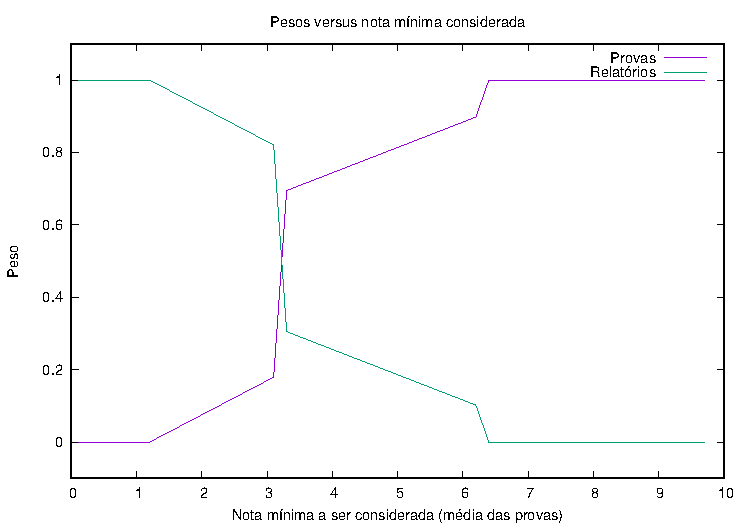
\includegraphics
                        [width=.8\linewidth]
                        {./img/domain_barrier/weights.pdf}
                        \caption{\small
                        Pesos para a média das provas
                        (em roxo) e dos relatórios
                        (em verde), em função da nota mínima
                        considerada para o método de mínimos
                        quadrados com a barreira de domínio.
                        Os valores numéricos dos pontos
                        presentes nesse gráfico podem ser
                        vistos na
                        Tabela~\ref{TAB_PESOS_MEDIA}.}
                        \label{FIG_DB_PESOS}
                \end{figure}
                \begin{figure}[!htp]
                        \centering
                        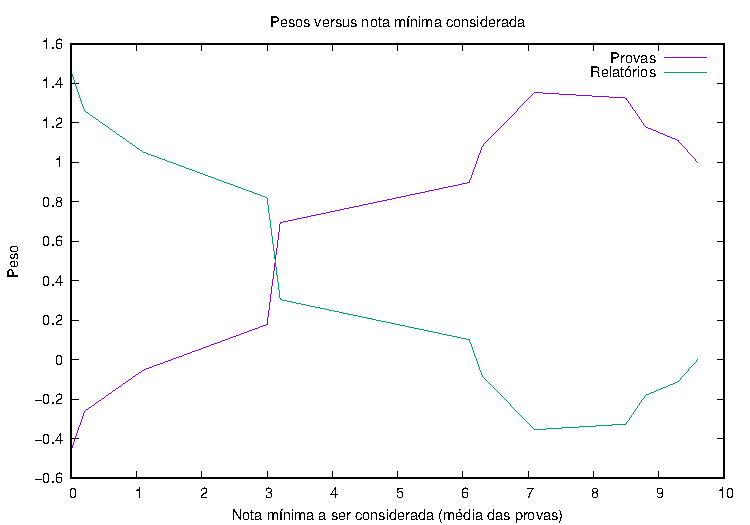
\includegraphics
                        [width=.8\linewidth]
                        {./img/no_barrier/weights.pdf}
                        \caption{\small
                        Pesos para a média das provas
                        (em roxo) e dos relatórios
                        (em verde), em função da nota mínima
                        considerada para o método de mínimos
                        quadrados sem a barreira de domínio.
                        Os valores numéricos dos pontos
                        presentes nesse gráfico podem ser
                        vistos na
                        Tabela~\ref{TAB_PESOS_MEDIA}.}
                        \label{FIG_NDB_PESOS}
                \end{figure}

                No caso dos pesos independentes, os valores
                encontrados para os pesos em função da
                nota de corte estão na
                Tabela~\ref{TAB_PESOS_INDEPENDENTES}
                e no gráfico da
                Figura~\ref{FIG_PESOS_INDEPENDENTES}.
                \begin{table}[!htp]
                        \centering
                        \begin{tabular}{c cccc}
        \hline
                      & \multicolumn{4}{c}{Pesos}\\ \cline{2-5}
        Nota de corte & Prova 1  & Prova 2 & Relatório 1
        & Relatório 2 \\
        \hline
        0    & 0.1386   & -0.414789  & 0.822417  & 0.453772  \\
        0.2  & 1.14185  & -0.744971  & -0.347389 & 0.950513  \\
        1.1  & 1.66639  & -0.756088  & -0.735138 & 0.824836  \\
        3    & 1.31196  & -0.437053  & -0.805813 & 0.93091   \\
        3.2  & 1.10159  & -0.135964  & -0.754942 & 0.789316  \\
        6.1  & 1.5482   & -0.304536  & -0.826339 & 0.582674  \\
        6.3  & 1.32118  & -0.0287221 & -0.761471 & 0.469017  \\
        7.1  & 0.672257 & 0.661219   & -0.368195 & 0.0347192 \\
        8.5  & 0.42029  & 0.86087    & -0.167391 & -0.113768 \\
        8.8  & 0.678161 & 0.448276   & 0.0775862 & -0.204023 \\
        9.3  & 0        & 1          & 0         & 0         \\
        \hline
\end{tabular}

                        \caption{\small
                        Tabela de pesos obtidos pela
                        configuração que leva em conta cada
                        avaliação independentemente.
                        Note que, diferentemente da
                        Tabela~\ref{TAB_PESOS_MEDIA}, em
                        nenhuma das notas de corte há apenas
                        pesos positivos. Isso ilustra a
                        dificuldade de aplicação desse método
                        para a maximização no caso em que
                        há múltiplos pesos independentes.
                        Um gráfico dos dados dessa tabela pode
                        ser visto na
                        Figura~\ref{FIG_PESOS_INDEPENDENTES}.
                        }
                        \label{TAB_PESOS_INDEPENDENTES}
                \end{table}

                \begin{figure}[!htp]
                        \centering
                        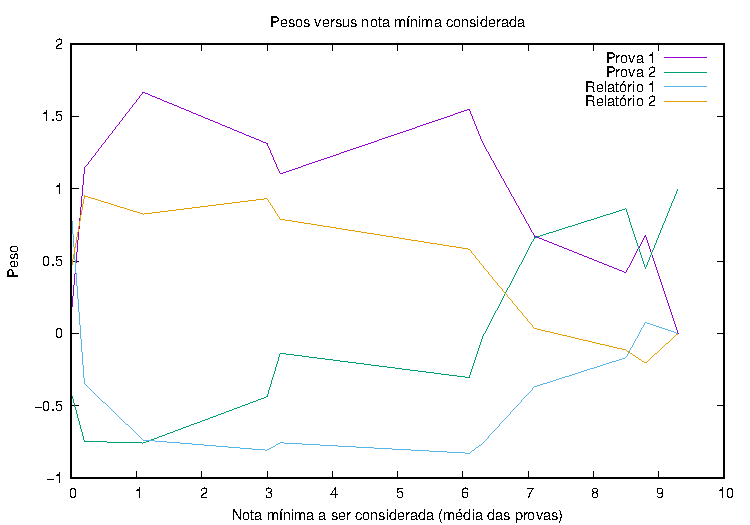
\includegraphics
                        [width=.8\linewidth]
                        {./img/independent/weights.pdf}
                        \caption{\small
                        Pesos para a prova $1$
                        (em roxo), para a prova $2$
                        (em verde), para o relatório $1$
                        (em azul) e para o relatório $2$
                        (em amarelo) em função da nota mínima
                        considerada para a média aritmética
                        das provas. Os dados numéricos desse
                        gráfico podem ser vistos na
                        Tabela~\ref{TAB_PESOS_INDEPENDENTES}.}
                        \label{FIG_PESOS_INDEPENDENTES}
                \end{figure}

                É importante notar que, embora no modelo
                de pesos para as médias dos relatórios e das
                provas existam três notas de corte para
                as quais são encontrados unicamente valores
                válidos, não há nenhuma nota de corte
                para a qual isso
                ocorra no modelo de pesos independentes.
                Isso sugere que, com mais pesos, a
                aplicação do método de mínimos quadrados
                exigindo restrições de domínio pode ser
                cada vez mais difícil de fornecer resultados
                frutíferos.

                Seguiu-se então uma análise do estado final
                da turma em termos de estudantes aprovados,
                em exame final ou reprovados. Os resultados
                numéricos dessa análise estão, para
                ambas as configurações e levando em conta
                tanto os casos com e sem barreira de domínio,
                na Tabela~\ref{TAB_STATUS_FINAL} e nos
                gráficos das
                Figuras~\ref{FIG_STATUS_BD}
                (pesos simples com barreira de domínio),
                \ref{FIG_STATUS_NBD}
                (pesos simples sem barreira de domínio) e
                \ref{FIG_STATUS_INDEPENDENTE}
                (pesos independentes).
                \begin{table}[!htp]
                        \centering
                        \begin{tabular}{c ccc ccc ccc}
        \hline
                      & \multicolumn{3}{c}{Médio com BD}
                      & \multicolumn{3}{c}{Médio sem BD}
                      & \multicolumn{3}{c}{Independentes} \\
                      \cline{2-10}
        Nota de corte & Apr. & Final & Rep.
                      & Apr. & Final & Rep.
                      & Apr. & Final & Rep. \\
        \hline
        0    & 13 & 1 & 1    & 10 & 5 & 0    & 11 & 4 & 0 \\
        0.2  & 13 & 1 & 1    & 10 & 5 & 0    & 12 & 2 & 1 \\
        1.1  & 13 & 1 & 1    &  9 & 5 & 1    & 11 & 3 & 1 \\
        3    & 11 & 3 & 1    & 11 & 3 & 1    & 11 & 2 & 2 \\
        3.2  &  9 & 4 & 2    &  9 & 4 & 2    & 11 & 2 & 2 \\
        6.1  &  9 & 2 & 4    &  9 & 2 & 4    & 10 & 3 & 2 \\
        6.3  &  9 & 2 & 4    &  7 & 4 & 4    & 10 & 3 & 2 \\
        7.1  &  9 & 2 & 4    &  7 & 4 & 4    &  9 & 2 & 4 \\
        8.5  &  9 & 2 & 4    &  7 & 4 & 4    &  7 & 4 & 4 \\
        8.8  &  9 & 2 & 4    &  7 & 4 & 4    &  7 & 4 & 4 \\
        9.3  &  9 & 2 & 4    &  7 & 4 & 4    &  7 & 4 & 4 \\
        9.6  &  9 & 2 & 4    &  9 & 2 & 4    &    &   &   \\
        \hline
\end{tabular}

                        \caption{\small
                        Tabela de estado final dos alunos
                        da disciplina em termos de alunos
                        aprovados, em exame final ou
                        reprovados para todas as configurações
                        de nota analisadas. Observe que a
                        última linha da coluna na configuração
                        de pesos independentes está faltando.
                        Isso ocorre pois, por possuir três
                        valores desconhecidos, o método de
                        mínimos quadrados não pode ser aplicado
                        quando a matriz das diferenças das
                        notas (ver
                        Equação~\ref
                        {LINEAR_PESOS_INDEPENDENTES})
                        possui menos de três linhas. À esta
                        tabela estão associados os gráficos das
                        Figuras~\ref{FIG_STATUS_BD},
                        \ref{FIG_STATUS_NBD} e
                        \ref{FIG_STATUS_INDEPENDENTE}.
                        As linhas destacadas correspondem
                        às linhas também destacadas na
                        Tabela~\ref{TAB_PESOS_MEDIA}, onde
                        todos os pesos da configuração
                        de pesos simples se apresentaram
                        positivos.}
                        \label{TAB_STATUS_FINAL}
                \end{table}

                \begin{figure}[!htp]
                        \centering
                        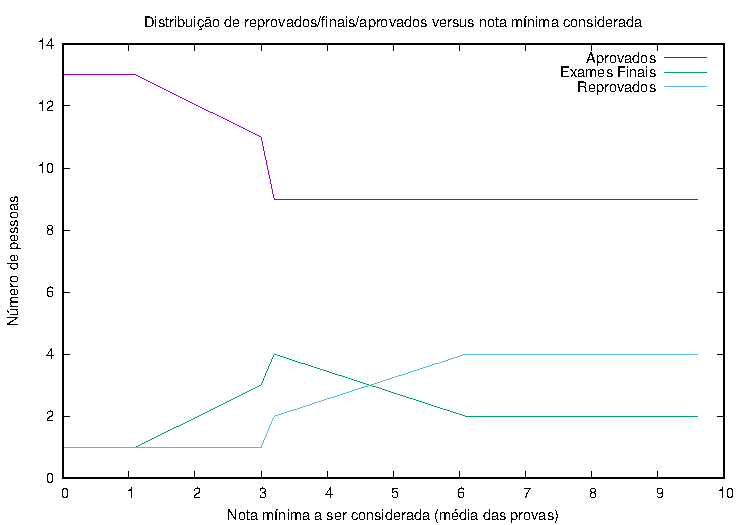
\includegraphics
                        [width=.8\linewidth]
                        {./img/domain_barrier/final_state.pdf}
                        \caption{\small
                        Gráfico do número de alunos
                        aprovados (em roxo), em exame final
                        (em verde) e reprovados (em azul)
                        para a configuração de pesos simples,
                        que leva em conta a nota média dos
                        relatórios e a nota média da prova,
                        com barreira de domínio, em função da
                        nota de corte mínima considerada para
                        o método de mínimos quadrados.}
                        \label{FIG_STATUS_BD}
                \end{figure}
                \begin{figure}[!htp]
                        \centering
                        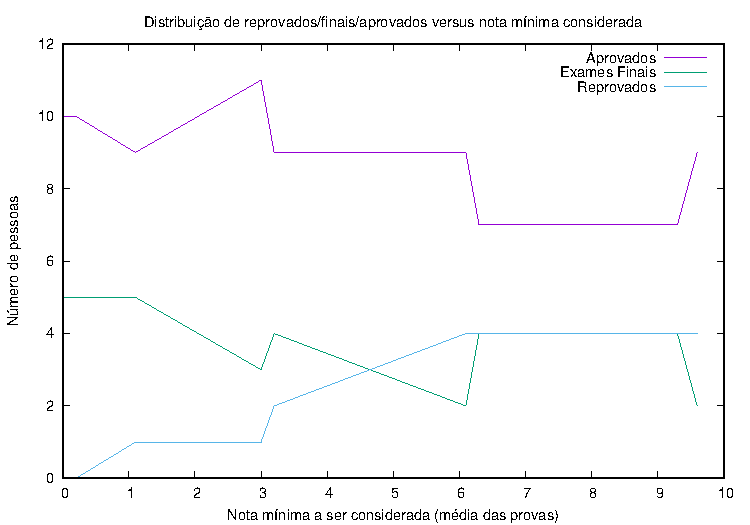
\includegraphics
                        [width=.8\linewidth]
                        {./img/no_barrier/final_state.pdf}
                        \caption{\small
                        Gráfico do número de alunos
                        aprovados (em roxo), em exame final
                        (em verde) e reprovados (em azul)
                        para a configuração de pesos simples,
                        que leva em conta a nota média dos
                        relatórios e a nota média da prova,
                        sem barreira de domínio, em função da
                        nota de corte mínima considerada para
                        o método de mínimos quadrados.}
                        \label{FIG_STATUS_NBD}
                \end{figure}
                \begin{figure}[!htp]
                        \centering
                        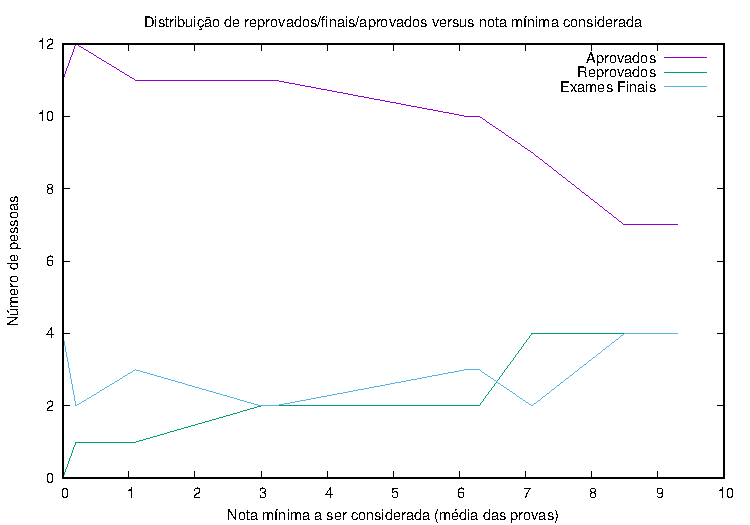
\includegraphics
                        [width=.8\linewidth]
                        {./img/independent/final_state.pdf}
                        \caption{\small
                        Gráfico do número de alunos
                        aprovados (em roxo), em exame final
                        (em verde) e reprovados (em azul)
                        para a configuração de pesos
                        independentes, em função da
                        nota de corte mínima considerada para
                        o método de mínimos quadrados.}
                        \label{FIG_STATUS_INDEPENDENTE}
                \end{figure}

                Nos gráficos das
                Figuras~\ref{FIG_STATUS_BD},
                \ref{FIG_STATUS_NBD} e
                \ref{FIG_STATUS_INDEPENDENTE}, e também na
                Tabela~\ref{TAB_STATUS_FINAL}, é possível
                observar que a configuração que atinge o maior
                número de aprovados é a média com barreira de
                domínios. Entretando, as duas outras são
                capazes (com pesos negativos) de encontrar
                configurações tais que nenhum aluno estaria
                imediatamente reprovado. É interessante
                observar também que, quando a nota de corte
                se torna maior do que zero, e os alunos com
                notas nulas nas provas passam a ser
                desconsiderados, há, na
                Figura~\ref{FIG_STATUS_INDEPENDENTE}, um
                aumento no número de aprovações, o que
                mostra que esses alunos são têm
                notas que destoam do padrão da turma.
                Foram destacadas as linhas que também estão
                destacadas na Tabela~\ref{TAB_PESOS_MEDIA},
                nas quais os pesos da configuração de pesos
                simples se apresentaram positivos.

                Outro fator a ser observado nesses gráficos é
                de que a maior liberdade para os pesos não
                implica necessariamente numa maior capacidade
                de aprovação, isto é, há mais notas altas
                na configuração de pesos simples com barreira
                de domínio.

                Finalmente, estudou-se também como se comporta
                a média da turma ao variarmos o limiar de
                nota. Os resultados estão na
                Tabela~\ref{TAB_MEDIA_FINAL} e no gráfico da
                Figura~\ref{FIG_MEDIA_FINAL}.

                \begin{table}[!htp]
                        \centering
                        \begin{tabular}{c ccc}
        \hline
                      & \multicolumn{3}{c}{Método} \\ \cline{2-4}
        Nota de corte & Média com BD & Média sem BD & Independentes \\
        \hline
        0    & 7.2     & 7.50143  & 7.54987 \\
        0.2  & 7.2     & 7.37301  & 7.84565 \\
        1.1  & 7.2     & 7.23458 & 7.74893  \\
        3    & 7.08109 & 7.08109 & 7.53332  \\
        3.2  & 6.73897 & 6.73897 & 7.24801  \\
        6.1  & 6.60445 & 6.60445 & 7.28547  \\
        6.3  & 6.53667 & 6.48256 & 7.0332   \\
        7.1  & 6.53667 & 6.30198 & 6.37349  \\
        8.5  & 6.53667 & 6.32048 & 6.18549  \\
        8.8  & 6.53667 & 6.41722 & 6.5049   \\
        9.3  & 6.53667 & 6.46296 & 6.14667  \\
        9.6  & 6.53667 & 6.53667 &          \\
        \hline
\end{tabular}

                        \caption{\small
                        Média da turma em função do limiar de
                        nota. As linhas destacadas correspondem
                        às linhas destacadas na
                        Tabela~\ref{TAB_PESOS_MEDIA},
                        quando os pesos da configuração de
                        pesos simples se mostraram positivos.
                        O gráfico correspondente a essa tabela
                        pode ser visto na
                        Figura~\ref{FIG_MEDIA_FINAL}.}
                        \label{TAB_MEDIA_FINAL}
                \end{table}

                \begin{figure}[!htp]
                        \centering
                        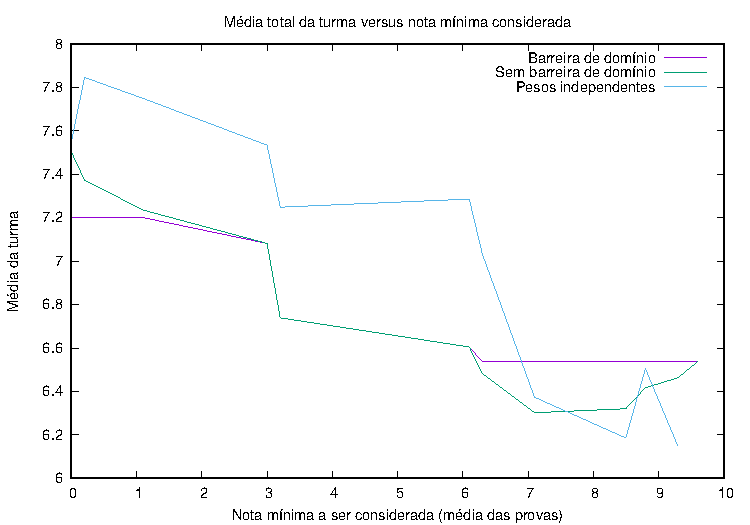
\includegraphics
                        {./img/together/total_class_average.pdf}
                        \caption{\small
                        Gráfico da média da turma para a
                        configuração de pesos simples com
                        barreira de domínio (em roxo),
                        sem barreira de domínio (em verde) e
                        com pesos independentes (em azul) em
                        função da nota mínima a ser
                        considerada. Os valores numéricos dos
                        pontos nesse gráfico estão na
                        Tabela~\ref{TAB_MEDIA_FINAL}.}
                        \label{FIG_MEDIA_FINAL}
                \end{figure}

                Observa-se na
                Tabela~\ref{TAB_MEDIA_FINAL} e na
                Figura~\ref{FIG_MEDIA_FINAL} que há uma
                vantagem com o uso dos pesos independentes:
                a média da turma se mantém significativamente
                acima quando comparada aos outros dois casos.
                De forma similar, a média da turma é
                superior
                quando os pesos não passam por uma
                barreira de domínio do que quando passam.
                Esse padrão continua até a região final do
                gráfico, quando são consideradas apenas
                notas acima de $6$, e a ordem dos gráficos
                passa a se inverter. Isso pode ser atribuído
                à redução do número de elementos para os
                quais a maximização está sendo feita, o que
                transmite aos pesos detalhes específicos
                de um único aluno, ao invés de considerar
                um padrão mais geral para a turma.
                Em especial, é possível notar pelo gráfico
                de pesos independentes uma ``volatilidade''
                maior, especialmente pela sua queda brusca
                quando a nota mínima passa de $6.0$ para
                $7.0$ e pelo pico entre as notas de
                $8.0$ e $9.0$, que; em consonãncia com a
                hipótese de que a redução do número de
                alunos para o qual a maximização é feita
                transmite ao resultado final detalhes
                individuais que não necessariamente correspondem
                a um padrão real no grupo todo; parece se
                dever a um aluno cuja configuração de
                notas destoa da turma, e que possui uma
                média das provas nessa faixa, e, quando
                removido, causa um salto na média da turma.

% Conclusões
        \section{Conclusões}
                Por meio dos resultados obtidos nessa
                aplicação empírica do método dos mínimos
                quadrados, constatou-se sua validade para
                situações desse contexto e de contexto
                semelhante.

                Valem, todavia, as ressalvas já apontadas no
                corpo do texto, em especial da dificuldade de
                estabelecer pesos válidos para o método quando
                há muitas variáveis independentes. Uma
                solução possível porém não empregada para esse
                problema seria uma extensão da barreira
                de domínio para que, quando um dos pesos
                fosse negativo ou nulo, desconsiderasse-se
                sua nota correspondente e fosse refeito com as
                demais notas o método de maximização levando
                em conta uma matriz de dimensões reduzidas.

                Contudo, o método de mostrou frutífero
                quando consideramos os pesos apenas para as
                médias aritméticas das provas e dos
                relatórios, para os quais, de acordo com a
                Tabela~\ref{TAB_PESOS_MEDIA}, há três
                estados (linhas destacadas) com ambos os
                pesos válidos. Algum desses pesos poderá então
                ser usado realmente na situação real para
                o cálculo das médias finais dos alunos.

                Curiosamente, na disciplina de Física
                Básica 2, a porcentagem do peso da média
                das provas e a porcentagem do peso da
                média dos relatórios usualmente utilizados é
                $70\%$ e $30\%$, respectivamente, o que está
                muito próximo do valor central entre os três
                valores destacados na
                Tabela~\ref{TAB_PESOS_MEDIA}. Isso sugere
                um possível padrão que poderá, em algum
                estudo futuro, ser analisado.

                Por fim, ressalta-se que o trabalho atingiu seu
                objetivo de atuar como
                \begin{otherlanguage}{english}
                        \textit{proof of concept}
                \end{otherlanguage}
                para a ideia de aplicação do método dos
                mínimos quadrados para maximização, na média,
                das notas de alunos de uma disciplina.
% Bibliografia
        \printbibliography
\end{document}
